
\subsection*{Opgave 1}

Den totale levetid for en bestemt pære antages at være normalfordelt med $\mu = 2000$ timer og $\sigma = 120$ timer.

\begin{enumerate}[label=\roman*)]
	\item Bestem sandsynligheden for at pæren lever kortere end 1800 timer.
	\item Bestem sandsynligheden for at pæren lever mellem 1900 og 2100 timer.
	\item Bestem sandsynligheden for at pæren lever mere end 2300 timer. 
\end{enumerate}

\subsection*{Opgave 2 (Uden Maple)}

En normalfordelt stokastisk variabel $X$ har følgende Gauss-kurve som tæthedsfunktion.
\begin{center}
	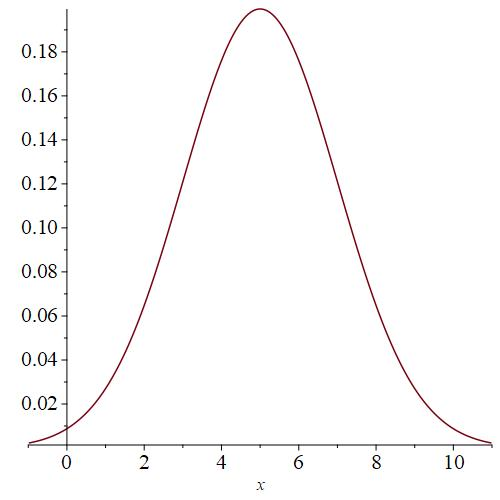
\includegraphics[width=0.7\textwidth]{Billeder/gauss.jpg}
\end{center}
Den har middelværdi $\mathbb{E}[X] = 5$. Det oplyses, at der for tæthedsfunktionen $f$ på figuren gælder, at
\begin{align*}
	\int_2^5f(x)dx = 0.433.
\end{align*}
Brug dette til at bestemme følgende sandsynligheder
\begin{enumerate}[label=\roman*)]
	\item $P(2<X<8)$.
	\item $P(X<2)$.
	\item $P(5<X)$.
	\item $P(8<X)$.
	\item $P(X=5)$.
\end{enumerate}


\subsection*{Opgave 3}

Intelligenskvotienten IQ er defineret til at være normalfordelt med $\mu = 100$ og $\sigma = 15$. 
\begin{enumerate}[label=\roman*)]
	\item Hvor mange mennesker lægger inden for én spredning fra middelværdien?
	\item For at være en del af MENSA-foreningen, der er en forening af mennesker med høj IQ skal du være blandt de 2 procent med højest IQ. Hvor høj skal din IQ være?
	\item Hvis man har en IQ på under 70, så vil man tildeles diagnosen udviklingshæmmet. Hvor stor en del af befolkningen vil have denne diagnose?
	\item Hvis IQ rent faktisk er normalfordelt, hvor mange i Danmark vil så have diagnosen udviklingshæmmet? (Der bor 5.9 mio i Danmark).
\end{enumerate}

\subsection*{Opgave 4}

På fødeafdelingen på et hospital har man skulle købe nye senge. En stor undersøgelse har vist, at højden på kvinder i Danmark er normalfordelt med $\mu = 167.1$ og $\sigma = 6.8$. De er enige om, at en seng er for kort, hvis den er mindre end 20cm længere end dig.
\begin{enumerate}[label=\roman*)]
	\item Hvor lange skal sengene mindst være, hvis 99$\%$ skal passe sengen?
\end{enumerate}



\subsection*{Opgave 5 (Uden Maple)}
	Af Fig. \ref{fig:fordeling} ses fordelingsfunktionerne $F$ og $G$ for to normalfordelte stokastiske variable
	\begin{align*}
		X \sim N(\mu,1)
	\end{align*}
	og 
	\begin{align*}
		Y \sim N(\mu,1.5).
	\end{align*}
	\begin{figure}[H]
		\centering
		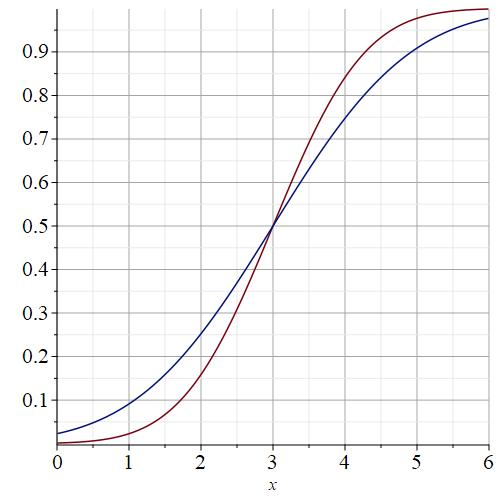
\includegraphics[width=0.7\textwidth]{Billeder/fordelingafl.jpg}
		\caption{Fordelingsfunktionerne $F$ og $G$.}
		\label{fig:fordeling}
	\end{figure}
\begin{enumerate}[label=\roman*)]
	\item Bestem middelværdien $\mu$ for de to stokastiske variable.
	\item Hvilken af de to kurver tilsvarer fordelingsfunktionen for henholdsvist $X$ og $Y$?
	\item Bestem sandsynlighederne
		\begin{align*}
			P(2<X<4) \textnormal{ og } P(1<Y).
		\end{align*}
\end{enumerate}
